% Matrix product state drawn as a tensor network (Session 4).
% Own drawing. Compile with: pdflatex mps_chain.tex ; result moves to ../mps_chain.pdf
\documentclass[11pt,tikz,border=3pt]{standalone}
\usepackage{amsmath,amssymb}
\usepackage{xcolor}
\definecolor{coursedark}{HTML}{1B2A4A}
\definecolor{courseaccent}{HTML}{7A2E8C}

\begin{document}
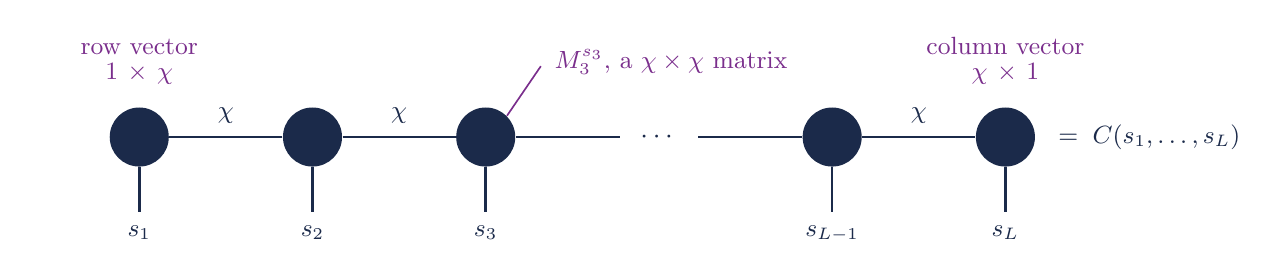
\begin{tikzpicture}[
    tensor/.style={circle, fill=coursedark, minimum size=7.5mm, inner sep=0pt},
    wire/.style={draw=coursedark, line width=0.9pt},
    lbl/.style={font=\small, text=coursedark},
  ]

  \def\legdrop{0.95}

  % ---- site tensors
  \foreach \i/\x/\s in {1/0/{s_1}, 2/2.2/{s_2}, 3/4.4/{s_3}, 4/8.8/{s_{L-1}}, 5/11.0/{s_L}} {
    \node[tensor] (t\i) at (\x,0) {};
    \draw[wire] (\x,-0.375) -- (\x,-\legdrop);
    \node[lbl, anchor=north] at (\x,-\legdrop-0.05) {$\s$};
  }

  % ---- bond legs between neighbouring tensors
  \draw[wire] (t1) -- (t2) node[lbl, midway, above=1pt] {$\chi$};
  \draw[wire] (t2) -- (t3) node[lbl, midway, above=1pt] {$\chi$};
  \draw[wire] (t4) -- (t5) node[lbl, midway, above=1pt] {$\chi$};

  % ---- the part of the chain we are not drawing
  \draw[wire] (t3) -- (6.1,0);
  \node[text=coursedark] at (6.6,0) {$\cdots$};
  \draw[wire] (7.1,0) -- (t4);

  % ---- what the whole contraction evaluates to
  \node[lbl, anchor=west, text=coursedark] at (11.55,0) {$=\;C(s_1,\ldots,s_L)$};

  % ---- what the two end tensors are
  \node[lbl, anchor=south, text width=2.6cm, align=center, text=courseaccent]
    at (0,0.55) {row vector\\[-2pt] $1\times\chi$};
  \node[lbl, anchor=south, text width=2.6cm, align=center, text=courseaccent]
    at (11.0,0.55) {column vector\\[-2pt] $\chi\times1$};

  % ---- what a bulk tensor is
  \node[lbl, anchor=west, text=courseaccent] at (5.15,0.95) {$M_3^{s_3}$, a $\chi\times\chi$ matrix};
  \draw[courseaccent, line width=0.6pt] (5.1,0.9) -- (4.67,0.27);

\end{tikzpicture}
\end{document}
